\documentclass[../main.tex]{subfiles}
%!TEX root = ./analysisFrictionWheelSlip.tex
\graphicspath {{../}}

\begin{document}
\subsection{Friction Wheel Slip} \label{frictionSlip}
\begin{figure}[H]
	\centering
	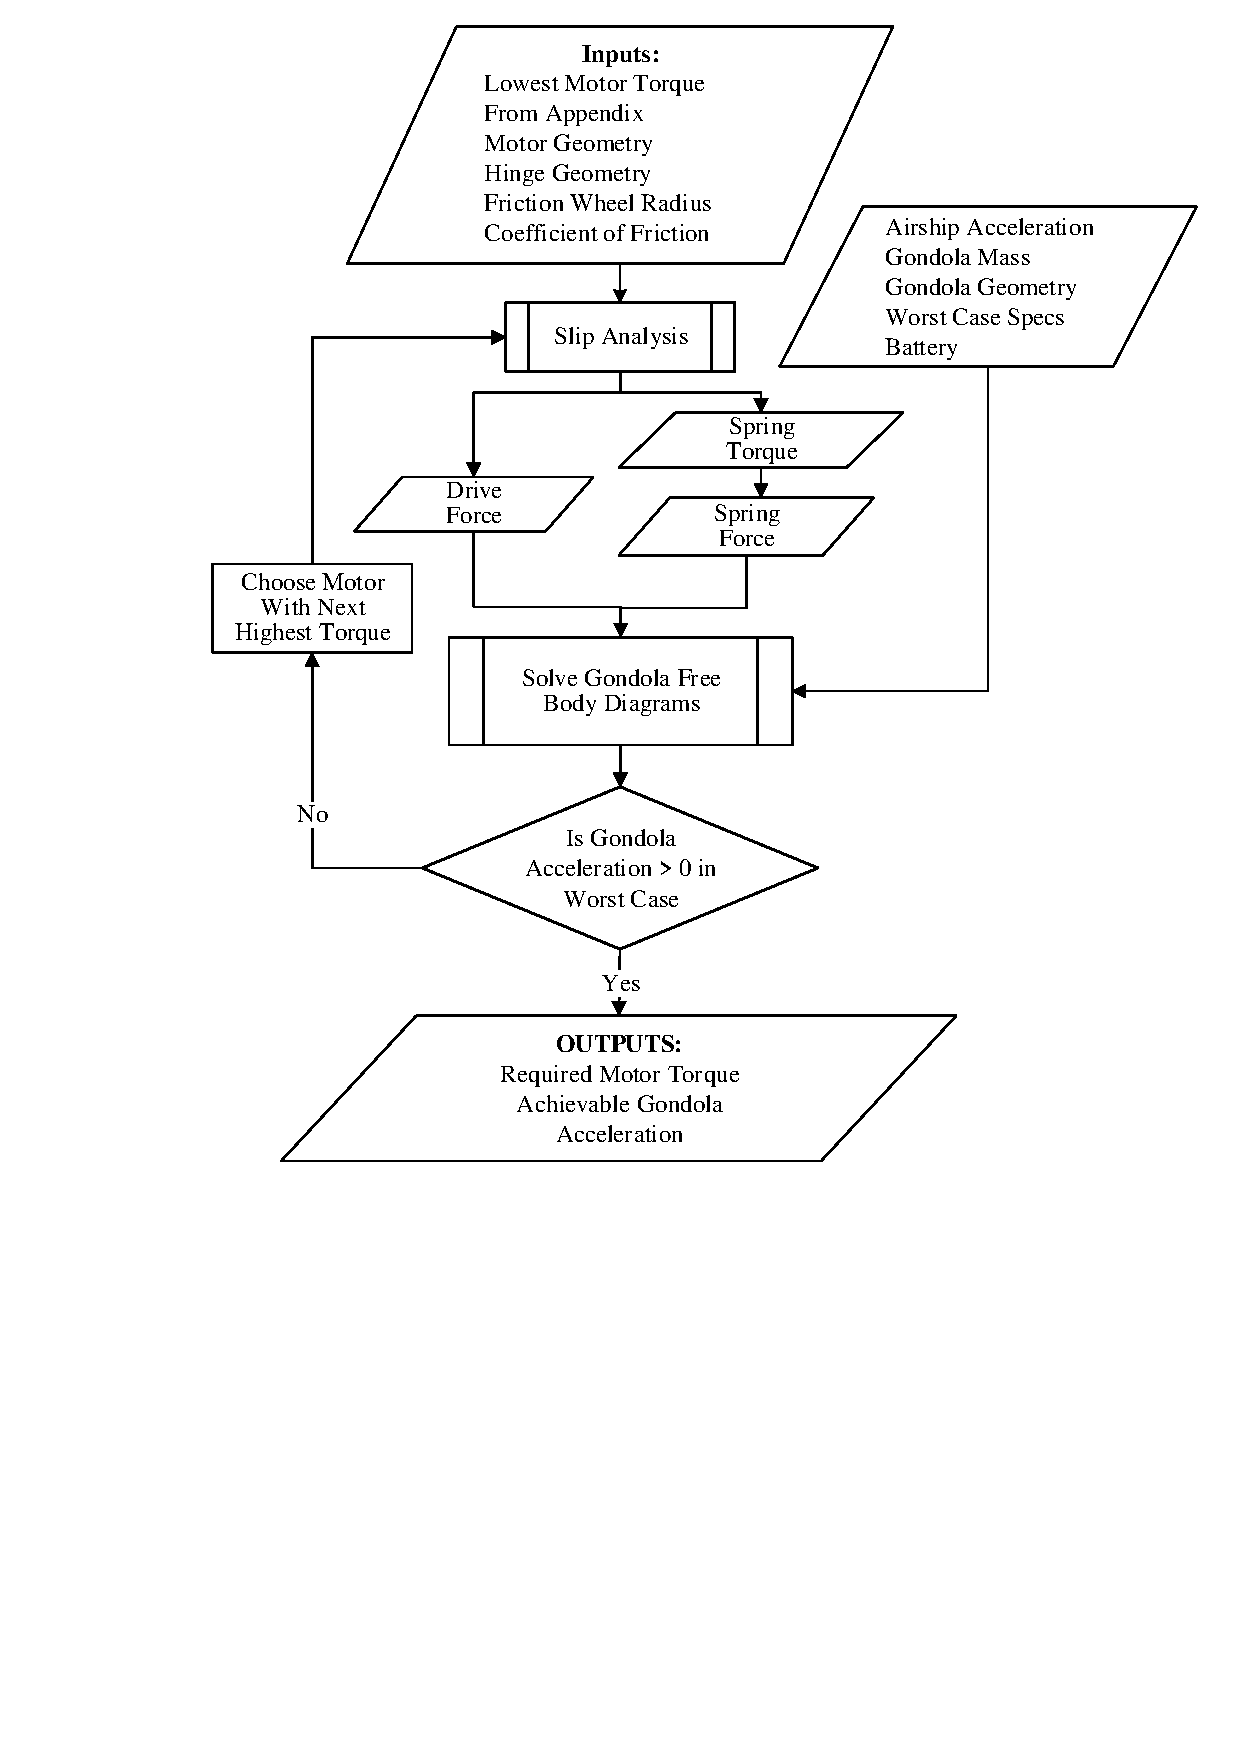
\includegraphics[width=.9\linewidth]{img/paramaterization/fricWheelSlip.pdf}
	\caption{Parametrization Outline for the Friction Wheel Slip}
	\label{fig:frictionWheelParametrization}
\end{figure}

The friction wheel slip analysis, calculates the required motor torque in order to allow for the gondola to move in a worst case scenario, and then calculates the motor hinge spring torque that will generate a large enough normal force to prevent slip of the friction wheel. The inputs required for the analysis are the geometry of the friction wheel, the motor, the hinge, the gondola, as well as the material properties of the friction wheel, the mass of each gondola car, the maximum achievable acceleration as a result of the thrusters and the loading conditions specific to the worst case scenario. \\

Parameters that will not change through out the gondola analysis include, the geometry of the motor, this is because different achievable torques with the same geometry by modifying the gearing. See Appendix \ref{FrictionMotor} for the specifications. The geometry of the hinge will not change as it is aluminium and the forces applied to it are minimal. The components inside of the gondola which include the RF transmitter, the BESC and the battery will not be changing. Calculations for required power and run time are done in the Component Analysis Section \ref{batterySelect}, Thruster Assembly Component Selection, show that regardless of motor gearing, power requirements are easily met and the limiting factor for flight time will be the thruster batteries. As a result the geometry of the main frame of the gondola (length, width, and height) will not be parametrized and the weights of the gondola will remains approximately the same. \\

The analysis first assumes a motor torque. With this torque, the code computes the spring torque such that $F_{spring} = F_{Nfric}$, which ensures the friction wheel will not slip. For the purpose of this analysis, the friction wheel and shaft interface are considered without slip, and the set screw is assumed to not fail as it will be metal interfacing with plastic.

\begin{equation}
F_{spring} = F_{Nfric} = \frac{F_{fFric}}{\mu} = \frac{T_w}{r_{Fw}\cdot{}\mu}
\end{equation}
\begin{equation}
\label{eqn:springForce}
F_{spring} = \frac{T_{spring}}{L_{hs}+L_{sw}}
\end{equation}
\begin{equation}
\frac{T_{spring}}{[L_{hs}+L_{sw}]} = \frac{T_w}{r_{Fw}\cdot{}\mu}
\end{equation}

The relation for the minimum necessary spring torque is multiplied by a factor of 1.5 in order to account for any neglected external factors.

\begin{equation}
\label{eqn:springTorque}
T_{spring} = \frac{T_w\cdot{\sqrt{L_{hs}^2+L_{sw}^2}}}{r_{Fw}\cdot{}\mu}\cdot{1.5}
\end{equation}

\begin{equation}
\label{eqn:driveForce}
F_{Drive} = \frac{T_w}{r_{Fw}}
\end{equation}

Based on the assumed torque and the spring force, the acceleration of the gondola in the worst case scenario explained in the System Modelling Section \ref{loadingScenarios}, Maximum Downward Force, and Figure \ref{fig:scenario1}, the acceleration of the gondola is calculated. The free body diagrams shown in Figures \ref{fig:gondolaSideTW} and \ref{fig:gondolaTopTW} depict all the forces that will be acting on the gondola for this scenario in the coordinate system defined by the plane of the surface of the rear gondola car. As a result most of the forces and reactions acting on the front gondola need to be rotated according to the angle of the hinge, $\Theta$ is the angle between the gondolas which is in this case equal zero. Similarly $\phi$ is the pitch angle of the airship which is equal and $\beta$ is the angle at which the acceleration due to thrust is acting. 
\begin{figure}[H]
	\centering
	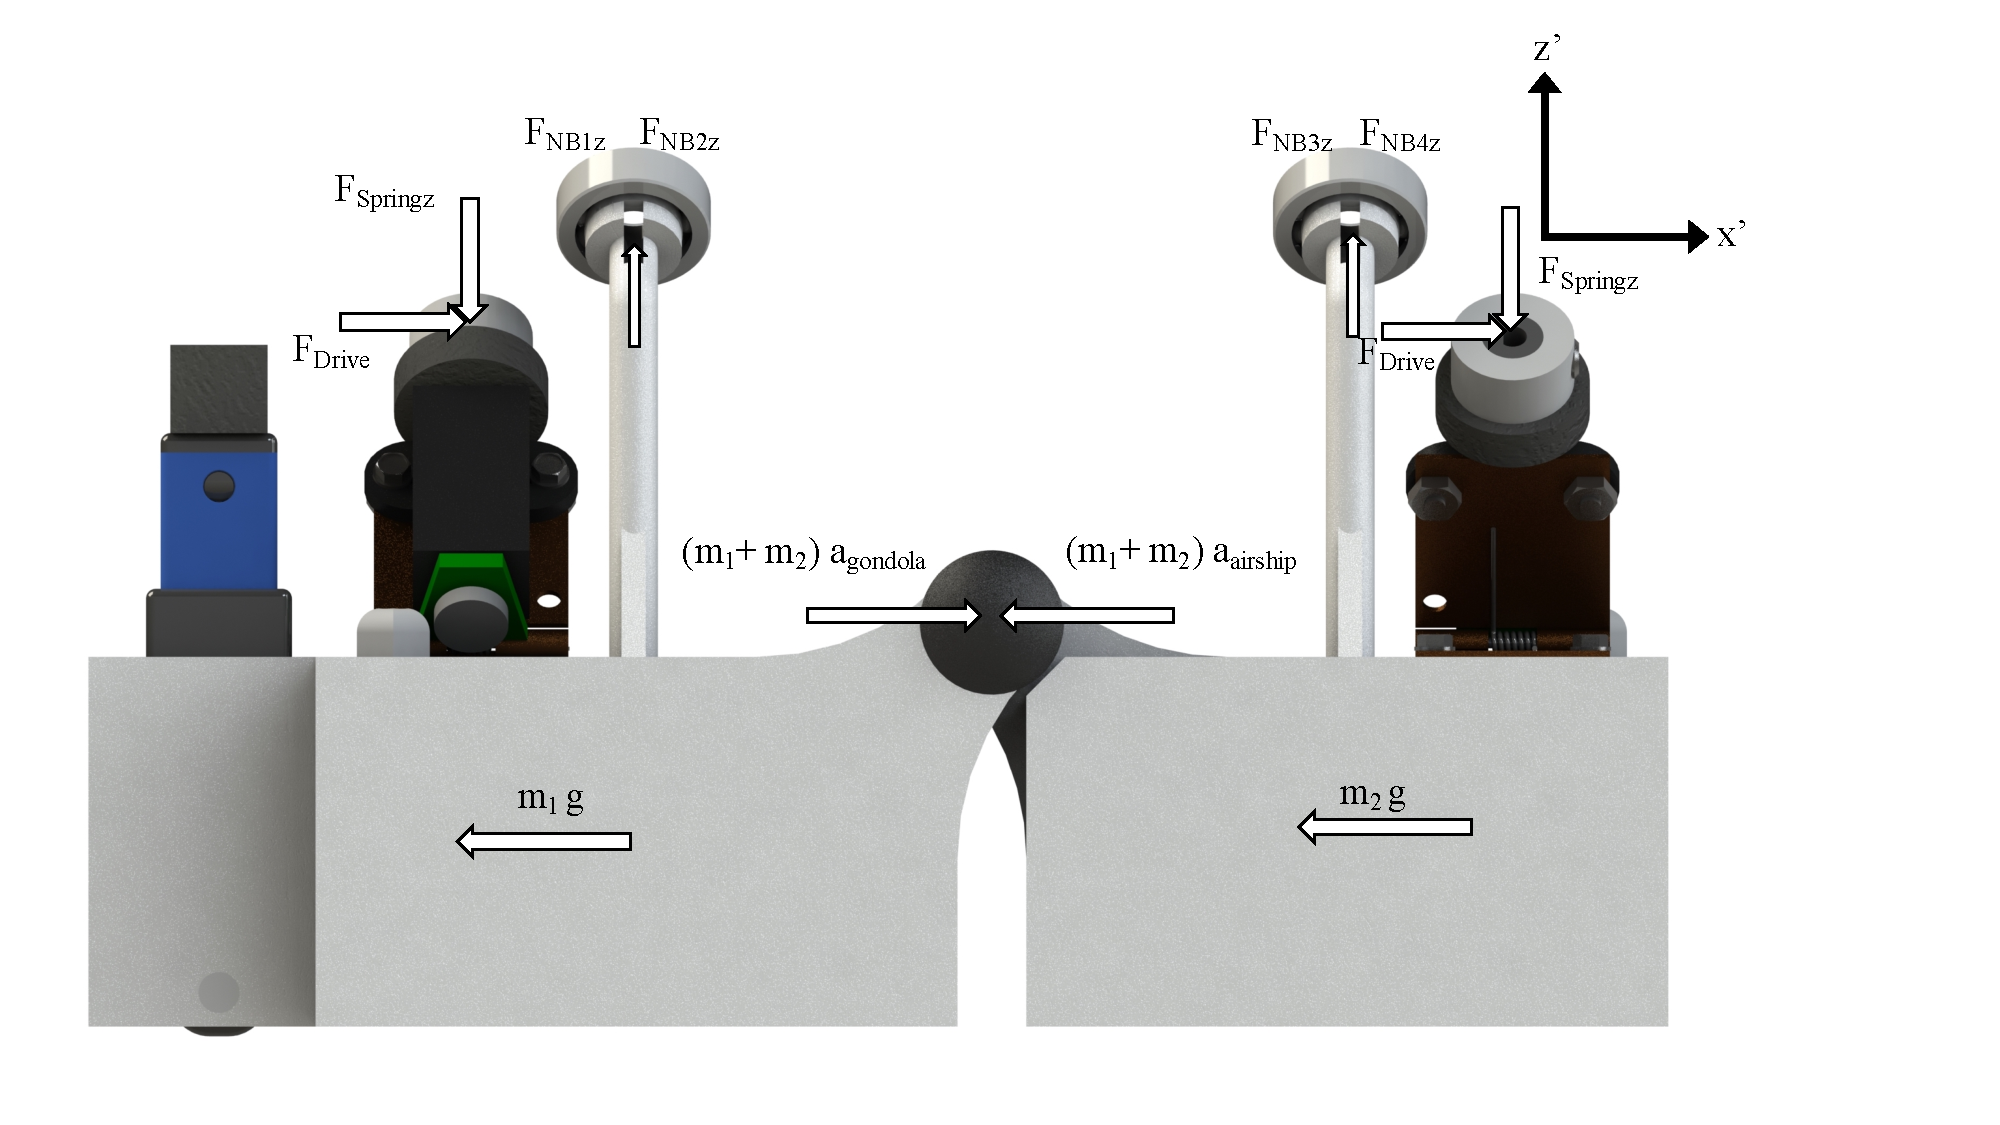
\includegraphics[width=1.1\linewidth]{img/gondola/gondolaSideTW.pdf}
	\caption{Side View of Gondola In Given Scenario}
	\label{fig:gondolaSideTW}
\end{figure}
\begin{figure}[H]
	\centering
	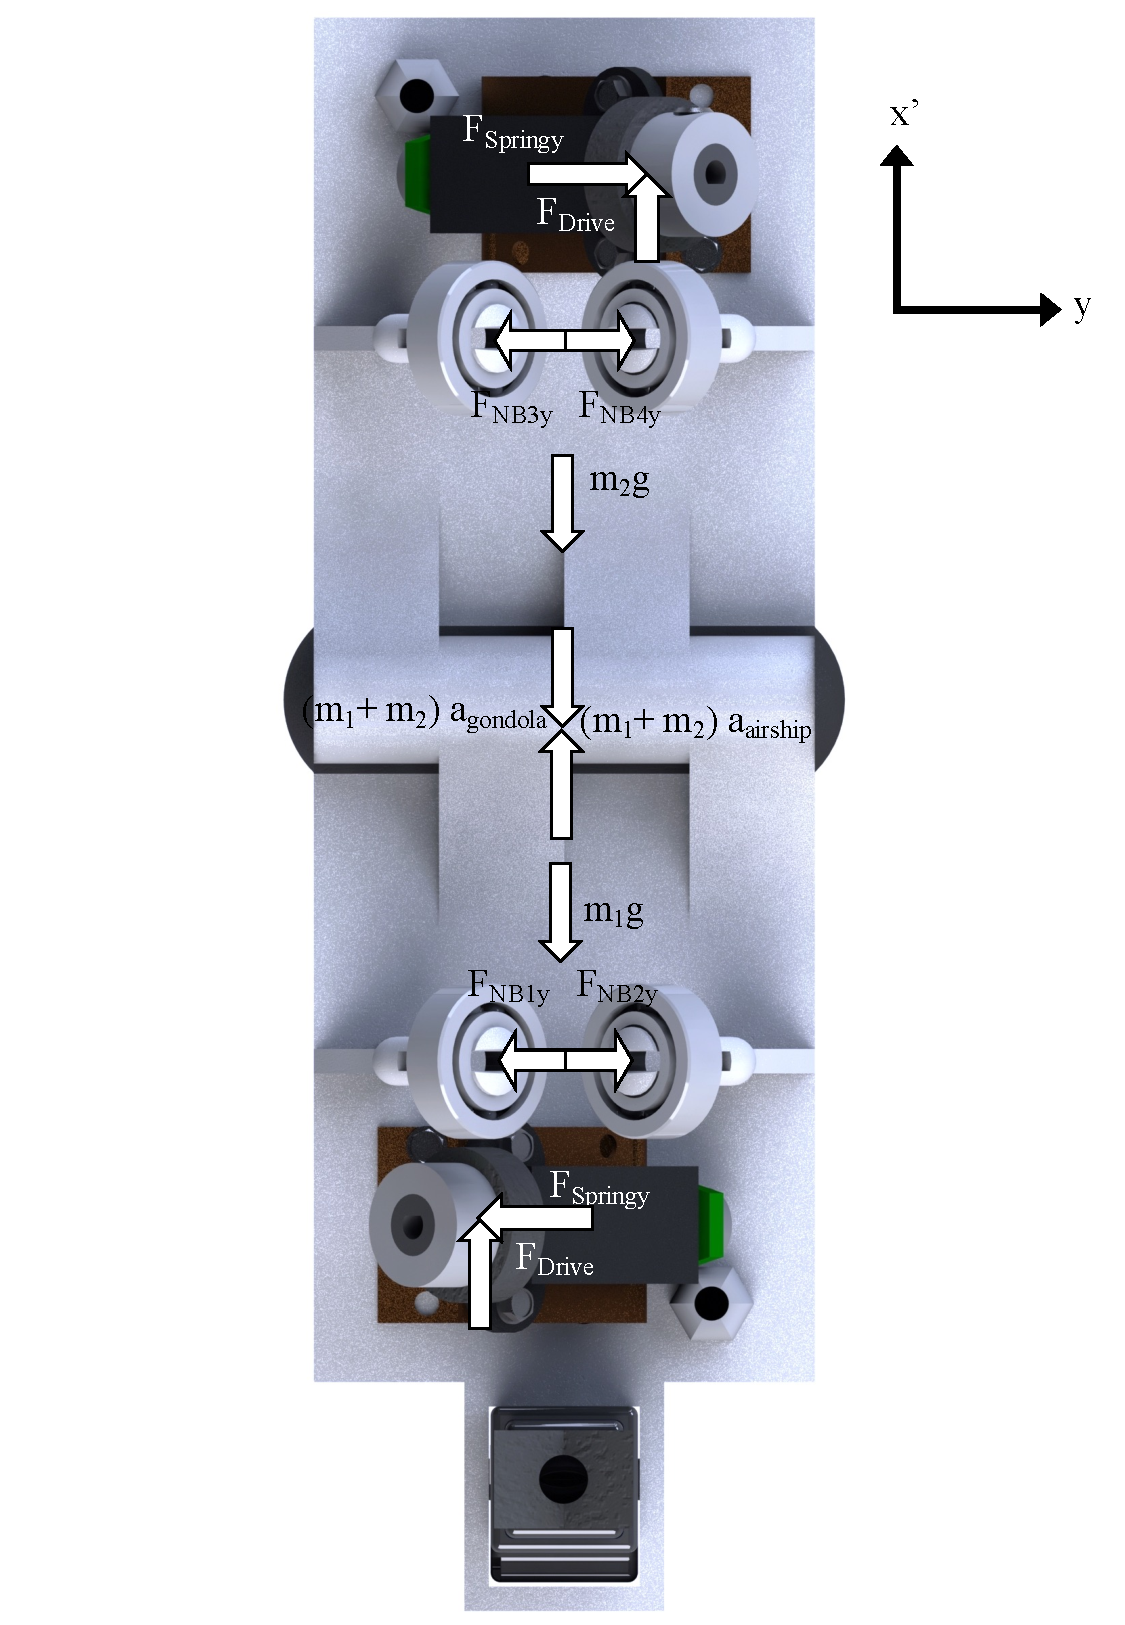
\includegraphics[width=1\textwidth]{img/gondola/gondolaTopTW.pdf}
	\caption{Top View of GondolaIn Given Scenario}
	\label{fig:gondolaTopTW}
\end{figure}

Equations \ref{Fxgondtw}, \ref{Fygondtw} and \ref{Fzgondtw} are the sum of forces acting on the gondola.
The reactions are on the left of the equal sign and the known forces acting on the gondola are to the right of the equal sign. 
\begin{multline} \label{Fxgondtw}
\Sigma F_{x} : (m_{1}+m_{2}) a_{gondola} = \sin(\phi)(m_{1} + m_2)g + F_{Drive} + F_{Drive} + \cos(\beta) (m_1+m_2) a_{Thrust} 
\end{multline}
\begin{flalign} \label{Fygondtw}
\hspace{12pt}\Sigma F_{y} : -F_{NB1_{y}} + F_{NB2_{y}} - F_{NB3_{y}} + F_{NB4_{y}} = F_{Springy} - F_{Springy} &&
\end{flalign}
\begin{multline} \label{Fzgondtw}
\Sigma F_{z} : F_{NB1_{z}} + F_{NB2_{z}} + F_{NB3_{z}} + F_{NB4_{z}} =\\ \cos(\phi) (m_{1} + m_2)g -  F_{Springz} - F_{Springz} + \sin(\beta) (m_1+m_2) a_{Thrust}+
\end{multline}
The spring forces $F_{Springz}$ and $F_{Springy}$ are acting on the keel at 45 \textdegree. The following equation can be used to define the spring forces. 
\begin{equation}
F_{Springz} = F_{Springy} = \frac{\sqrt{2}}{2} F_{Spring}
\end{equation}

With the GUI inputs specified in the System Modelling Section \ref{sampleCalcs} Sample Calculation Conditions, the calculated required motor torque $T_w$ was equal 0.0636[Nm]. For this motor torque the other results of the analysis are shown below:
\begin{equation*}
T_{spring} = \frac{T_w\cdot{}\sqrt{L_{hs}^2+L_{sw}^2}}{r{F_w}\cdot{}\mu}\cdot{}1.5 = \frac{0.0636[Nm]\cdot{\sqrt{(0.0219[m])^2+(0.0211[m])^2}}}{0.0127[m]\cdot{0.65}}\cdot{1.5} = 0.351[Nm]
\end{equation*}

\begin{equation*}
F_{Drive} = \frac{T_w}{r_{Fw}} =  \frac{0.0636[Nm]}{0.0127[m]} = 5.0043[N]
\end{equation*}

With this drive force in the worst case scenario with motors will be capable of at 4.64[$\dfrac{m}{s^2}$]. This is determined using the \textit{gondolaForces} code explained in the System Modelling Section \ref{gondForces}. 
\end{document}